\documentclass[a4paper, 14pt,russian]{article}
\usepackage[utf8x]{inputenc}
\usepackage[T2A]{fontenc}
\usepackage[russian]{babel}
\usepackage{hyperref}
\usepackage{indentfirst} % включить отступ у первого абзаца
\usepackage{listings}
\usepackage{color}
\usepackage{here}
\usepackage{cmap}          % русский поиск в pdf

\usepackage{times}
\renewcommand{\rmdefault}{ftm}

\usepackage{graphicx}
\graphicspath{{pic/}}
\lstset{inputpath=../listings}

\usepackage{caption}
\renewcommand{\lstlistingname}{Листинг}

\frenchspacing

\usepackage{listings}

\makeatletter
\DeclareRobustCommand{\getlstname}{%
	\begingroup
	% \lstname seems to change hyphens into \textendash
	\def\textendash{-}%
	\filename@parse{\lstname}%
	\texttt{\filename@base.\filename@ext}%
	\endgroup
}
\makeatother


\lstset{
	literate={а}{{\selectfont\char224}}1
	{б}{{\selectfont\char225}}1
	{в}{{\selectfont\char226}}1
	{г}{{\selectfont\char227}}1
	{д}{{\selectfont\char228}}1
	{е}{{\selectfont\char229}}1
	{ё}{{\"e}}1
	{ж}{{\selectfont\char230}}1
	{з}{{\selectfont\char231}}1
	{и}{{\selectfont\char232}}1
	{й}{{\selectfont\char233}}1
	{к}{{\selectfont\char234}}1
	{л}{{\selectfont\char235}}1
	{м}{{\selectfont\char236}}1
	{н}{{\selectfont\char237}}1
	{о}{{\selectfont\char238}}1
	{п}{{\selectfont\char239}}1
	{р}{{\selectfont\char240}}1
	{с}{{\selectfont\char241}}1
	{т}{{\selectfont\char242}}1
	{у}{{\selectfont\char243}}1
	{ф}{{\selectfont\char244}}1
	{х}{{\selectfont\char245}}1
	{ц}{{\selectfont\char246}}1
	{ч}{{\selectfont\char247}}1
	{ш}{{\selectfont\char248}}1
	{щ}{{\selectfont\char249}}1
	{ъ}{{\selectfont\char250}}1
	{ы}{{\selectfont\char251}}1
	{ь}{{\selectfont\char252}}1
	{э}{{\selectfont\char253}}1
	{ю}{{\selectfont\char254}}1
	{я}{{\selectfont\char255}}1
	{А}{{\selectfont\char192}}1
	{Б}{{\selectfont\char193}}1
	{В}{{\selectfont\char194}}1
	{Г}{{\selectfont\char195}}1
	{Д}{{\selectfont\char196}}1
	{Е}{{\selectfont\char197}}1
	{Ё}{{\"E}}1
	{Ж}{{\selectfont\char198}}1
	{З}{{\selectfont\char199}}1
	{И}{{\selectfont\char200}}1
	{Й}{{\selectfont\char201}}1
	{К}{{\selectfont\char202}}1
	{Л}{{\selectfont\char203}}1
	{М}{{\selectfont\char204}}1
	{Н}{{\selectfont\char205}}1
	{О}{{\selectfont\char206}}1
	{П}{{\selectfont\char207}}1
	{Р}{{\selectfont\char208}}1
	{С}{{\selectfont\char209}}1
	{Т}{{\selectfont\char210}}1
	{У}{{\selectfont\char211}}1
	{Ф}{{\selectfont\char212}}1
	{Х}{{\selectfont\char213}}1
	{Ц}{{\selectfont\char214}}1
	{Ч}{{\selectfont\char215}}1
	{Ш}{{\selectfont\char216}}1
	{Щ}{{\selectfont\char217}}1
	{Ъ}{{\selectfont\char218}}1
	{Ы}{{\selectfont\char219}}1
	{Ь}{{\selectfont\char220}}1
	{Э}{{\selectfont\char221}}1
	{Ю}{{\selectfont\char222}}1
	{Я}{{\selectfont\char223}}1
}

\lstdefinestyle{base_listing}{ %
	basicstyle=\footnotesize,       % the size of the fonts that are used for the code
	numbers=left,                   % where to put the line-numbers
	numberstyle=\footnotesize,      % the size of the fonts that are used for the line-numbers
	stepnumber=1,                   % the step between two line-numbers. If it is 1 each line will be numbered
	numbersep=5pt,                  % how far the line-numbers are from the code
	backgroundcolor=\color{white},  % choose the background color. You must add \usepackage{color}
	showspaces=false,               % show spaces adding particular underscores
	showstringspaces=false,         % underline spaces within strings
	showtabs=false,                 % show tabs within strings adding particular underscores
	frame=single,           % adds a frame around the code
	tabsize=2,          % sets default tabsize to 2 spaces
	captionpos=b,           % sets the caption-position to bottom
	breaklines=true,        % sets automatic line breaking
	breakatwhitespace=false,    % sets if automatic breaks should only happen at whitespace
	escapeinside={\%*}{*)},          % if you want to add a comment within your code
	postbreak=\raisebox{0ex}[0ex][0ex]{\ensuremath{\color{red}\hookrightarrow\space}},
	extendedchars=\true
}

\usepackage[left=2.5cm, top=2cm, right=2cm, bottom=2cm, nohead]{geometry}

\begin{document}
\begin{titlepage} % начало титульной страницы

\begin{center} % включить выравнивание по центру

\large Санкт-Петербургский Политехнический Университет Петра Великого\\
\large Институт компьютерных наук и технологий \\
\large Кафедра компьютерных систем и программных технологий\\[6cm]
% название института, затем отступ 4,5см

\huge Защита информации\\[0.5cm] % название работы, затем отступ 0,6см
\large Отчет по лабораторной работе №1\\[0.1cm]
\large Исследование сетевого трафика\\[5cm]
% тема работы, затем отступ 3,7см
\end{center}

\begin{flushright}
\begin{minipage}{0.5\textwidth}
\begin{flushright}
\textbf{Работу выполнил:}

Раскин Андрей

{Группа:} 43501/3\\


\textbf{Преподаватель:} 

Новопашенный Андрей Гелиевич 
\end{flushright}
\end{minipage} % конец врезки
\end{flushright} % конец выравнивания по левому краю

\vfill % заполнить всё доступное ниже пространство

\begin{center}

\large Санкт-Петербург\\
\large \the\year % вывести дату

\end{center} % закончить выравнивание по центру

\thispagestyle{empty} % не нумеровать страницу
\end{titlepage} % конец титульной страницы

\vfill % заполнить всё доступное ниже пространство

\section{Цель работы}
Закрепление навыков работы в программе WireShark и знаний о некоторых сетевых протоколах. 

\section{Программа работы}
При помощи анализатора сетевого трафика WireShark продемонстрировать в сети работу протокола
FTP:
\begin{enumerate}
	\item пассивный режим,
	\item активный режим,
	\item безопасность протокола.
\end{enumerate}

\section{Конфигурация компьютера в сети}
\begin{figure}[h]
	\center{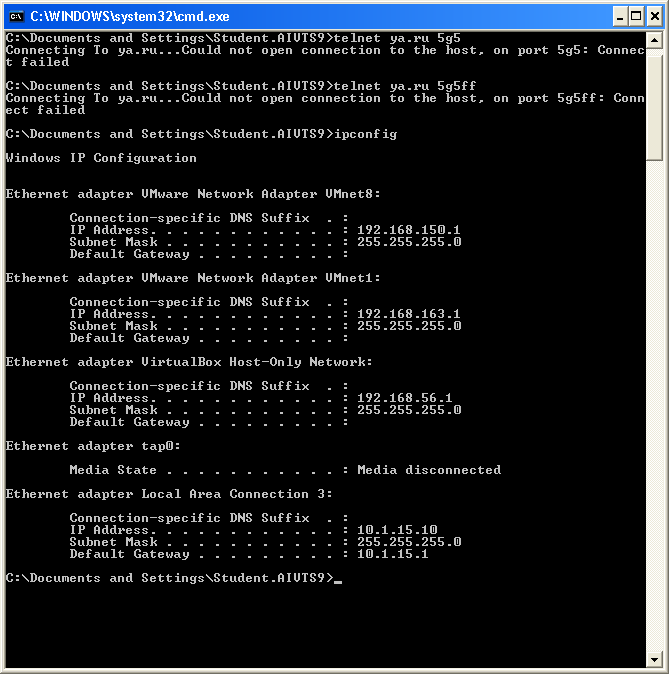
\includegraphics[scale=0.50]{ipconfig}}
	\caption{Конфигурация сети}
	\label{img:system}
\end{figure}

\section{Ход работы}

\subsection{Протокол FTP}
	Имеется два режима – активный и пассивный. В первом случае клиент создает управляющее соединение и ждет, когда сервер запустит TCP-соединение с заданными адресом и номером порта. В пассивном режиме, когда клиент не может принять входящее TCP-соединение, клиент отправляет серверу команду PASV, получает от сервера его IP-адрес и номер порта, которые затем использует для открытия потока данных с произвольного клиентского порта к полученным адресу и порту сервера.
	
\subsection{Пассивный режим}
	\begin{figure}[h!]
		\center{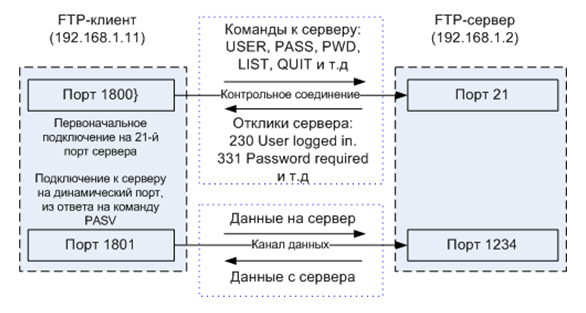
\includegraphics[scale=0.8]{passive_sheme}}
		\caption{Схема работы протокола ftp в пассивном режиме}
		\label{img:ftp_scheme}
	\end{figure}
	

	Клиент запрашивает у сервера переход в пассивный режим командой PASV, перед этим подключившись к серверу по TCP через 21й порт и авторизовавшись.
	
	\begin{figure}[h!]
		\center{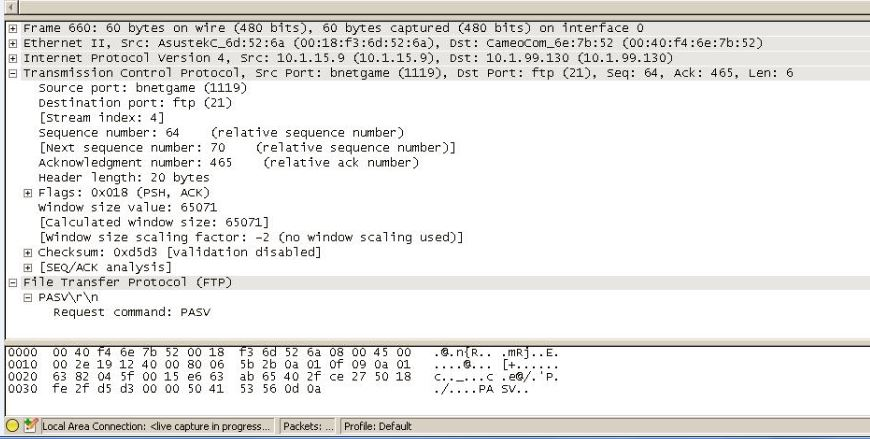
\includegraphics[scale=0.7]{ftp_passiven}}
		\caption{Запрос от клиента на установку соединения}
		\label{img:ftp_scheme}
	\end{figure}

	\newpage
	В ответ на команду PASV сервер передает клиенту IP адрес и 2 числа, из которых вычисляется номер порта для подключения к серверу.
	
	\begin{figure}[h!]
		\center{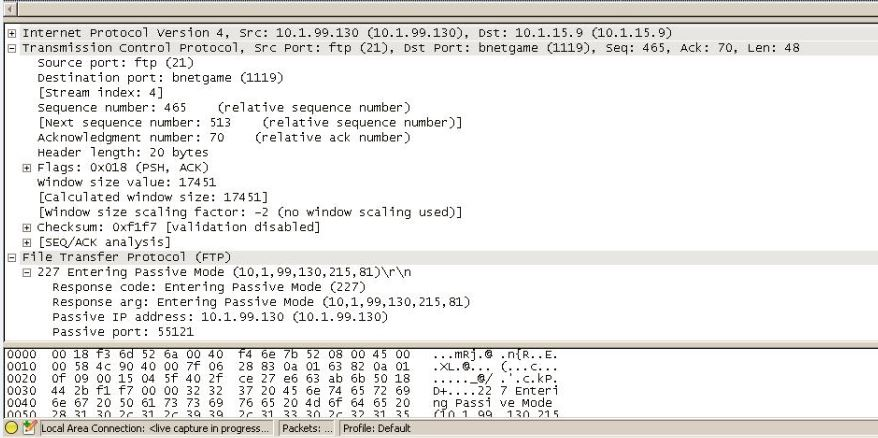
\includegraphics[scale=0.7]{ftp_passive2n}}
		\caption{Ответ сервера на команду PASV}
		\label{img:ftp_scheme}
	\end{figure}
	
	Затем осуществляется подключение по данным IP адресу и номеру порта. 
	\begin{figure}[h!]
		\center{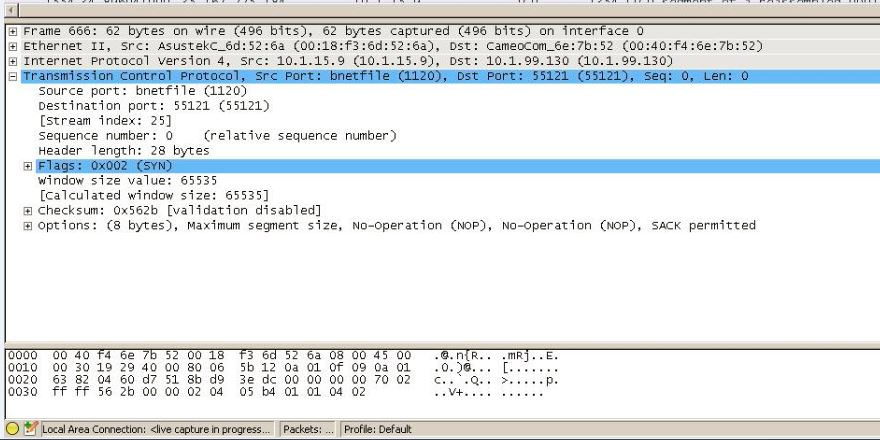
\includegraphics[scale=0.7]{ftp_passive3n}}
		\caption{Запрос на установку TCP-соединения}
		\label{img:ftp_scheme}
	\end{figure}
	
	Рассмотрим пример передачи файла в пассивном режиме. Для этого существует команда \textbf{RETR {файл}}
	Команды RETR, STOR и LIST можно прервать в процессе выполнения с помощью команды ABOR, в ответ на которую сервер должен ответить 426 «передача прервана», а затем — 226 «отмена операции произошла успешно».
	\newpage
	
	\begin{figure}[h!]
		\center{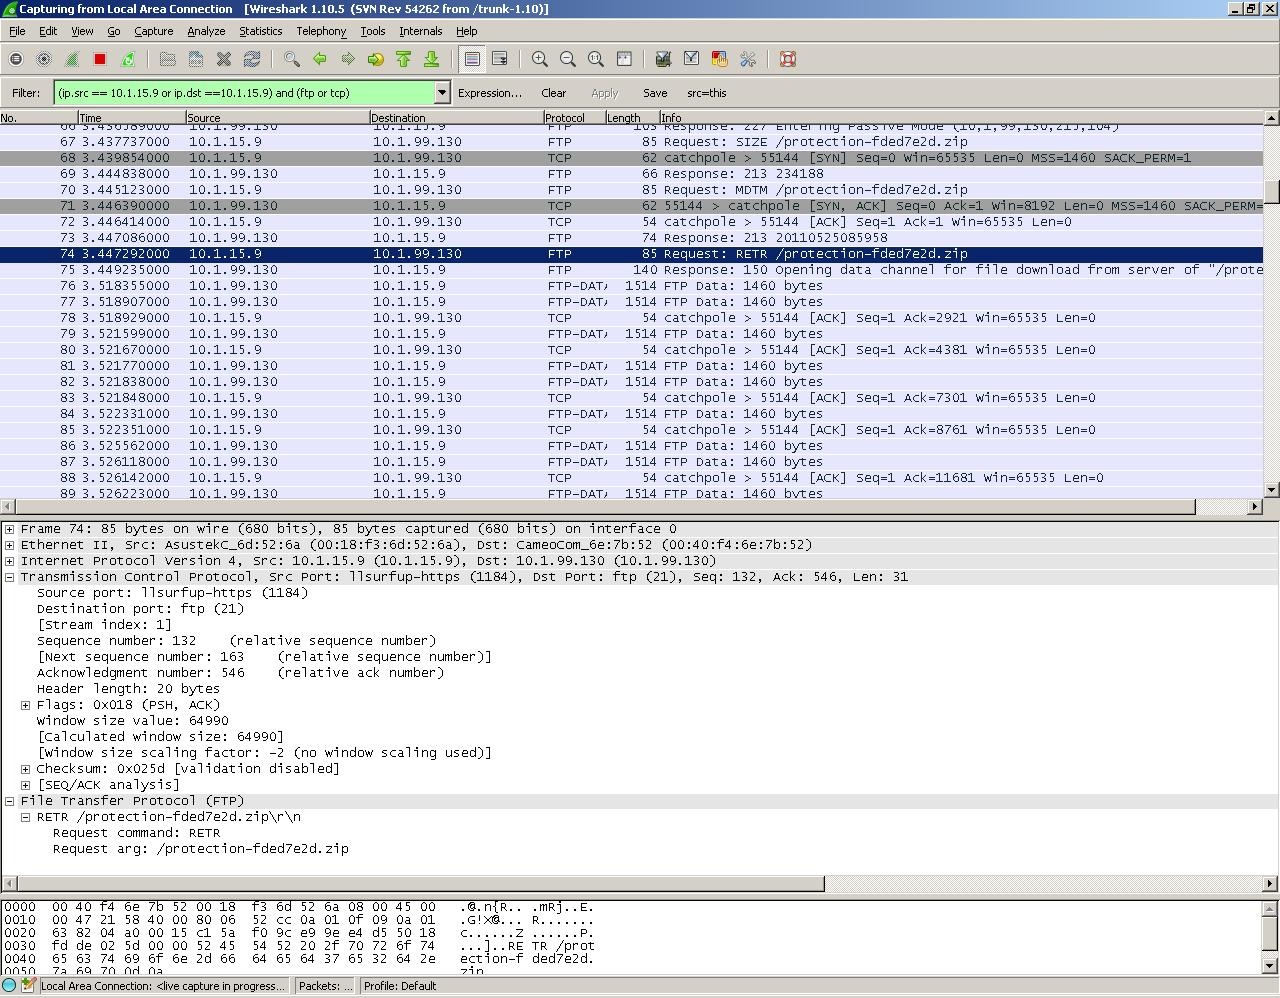
\includegraphics[scale=0.5]{ftp_file3}}
		\caption{Запрос на скачивание файла}
		\label{img:ftp_scheme}
	\end{figure}

	\begin{figure}[h!]
		\center{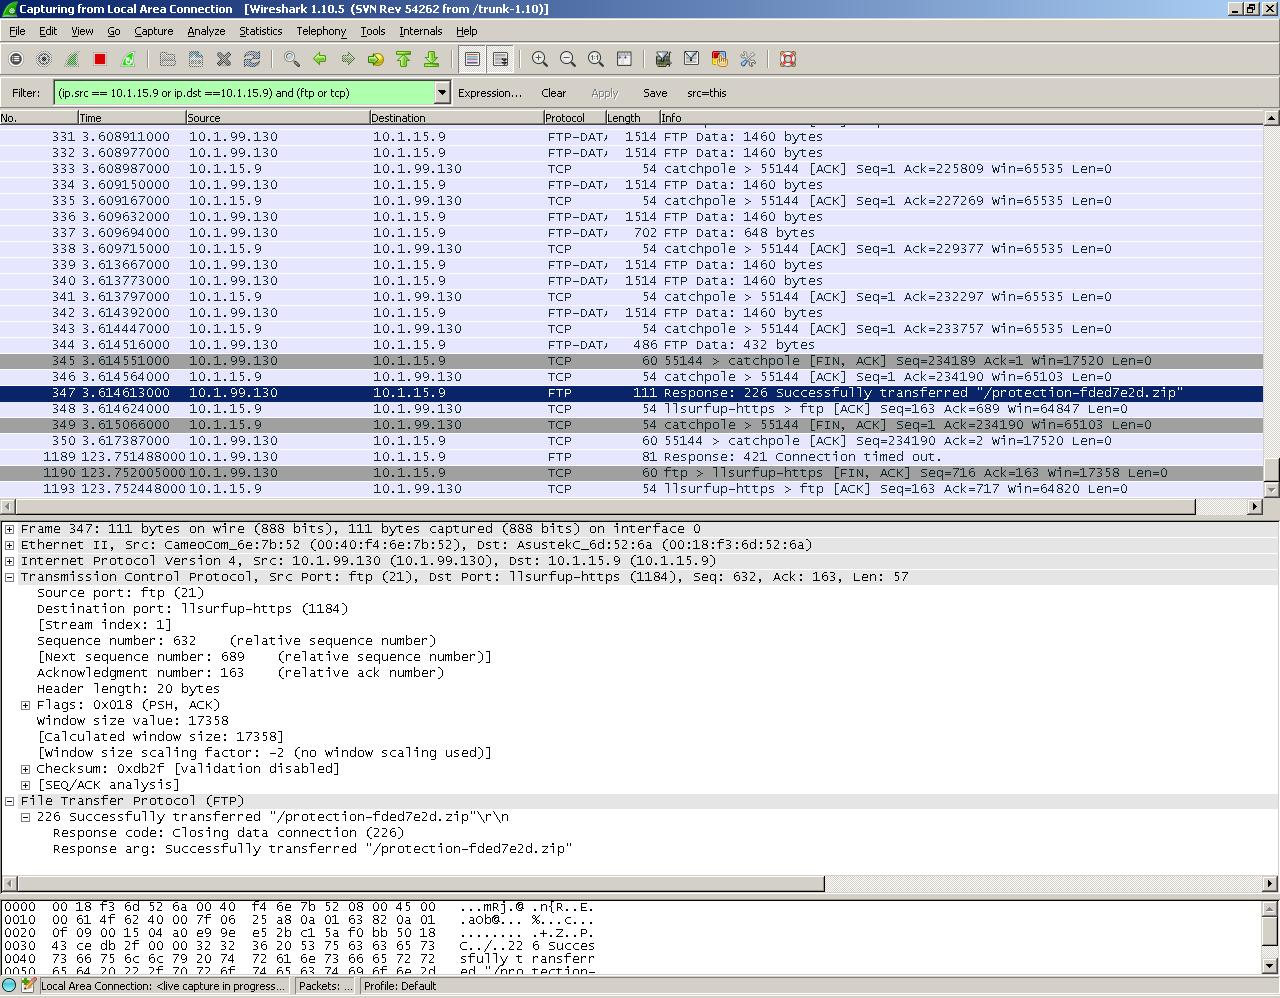
\includegraphics[scale=0.5]{ftp_file4}}
		\caption{Подтверждение получения файла}
		\label{img:ftp_scheme}
	\end{figure}
\newpage


\subsection{Активный режим}	

	\begin{figure}[h!]
		\center{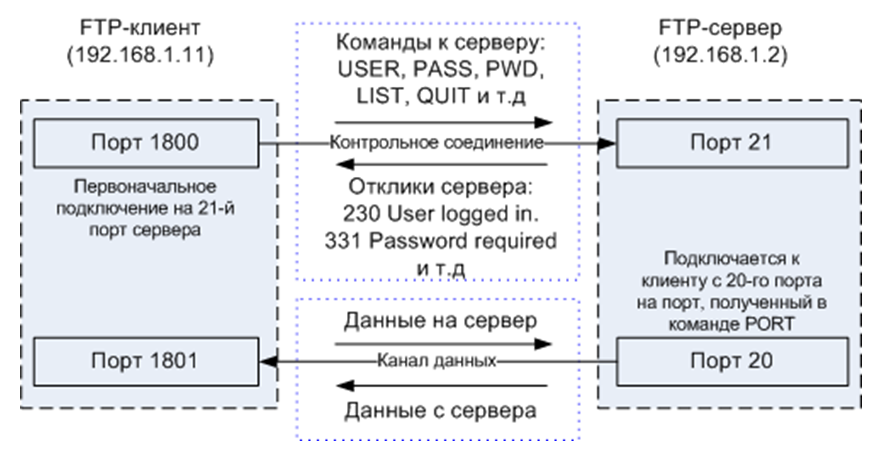
\includegraphics[scale=0.7]{active_sheme}}
		\caption{Схема работы протокола ftp в активном режиме}
		\label{img:ftp_scheme}
	\end{figure}

	Запрос на соединение от клиента. Содержит IP-адрес для подключения и два числа, из которых находится номер порта.
	
	\begin{figure}[h!]
		\center{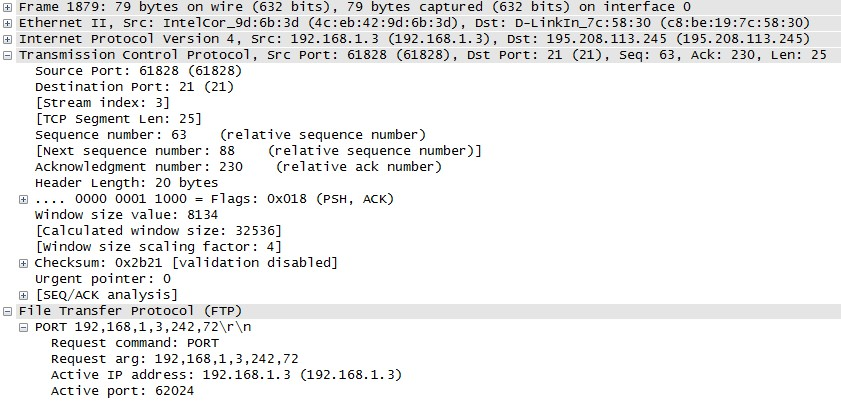
\includegraphics[scale=0.7]{port}}
		\caption{Пакет, содержащий команду PORT}
		\label{img:ftp_act1}
	\end{figure}
	
	
	
	\begin{figure}[h!]
	\center{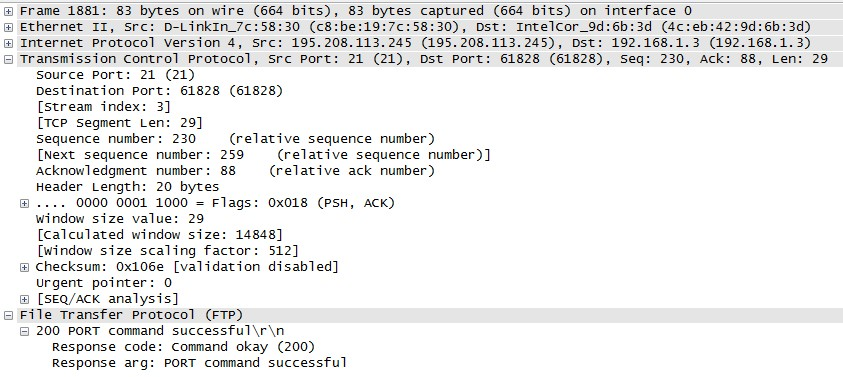
\includegraphics[scale=0.7]{portok}}
	\caption{Ответ об успешном выполнении команды}
	\label{img:ftp_act1}
	\end{figure}
	
	\newpage
	\begin{figure}[h!]
	\center{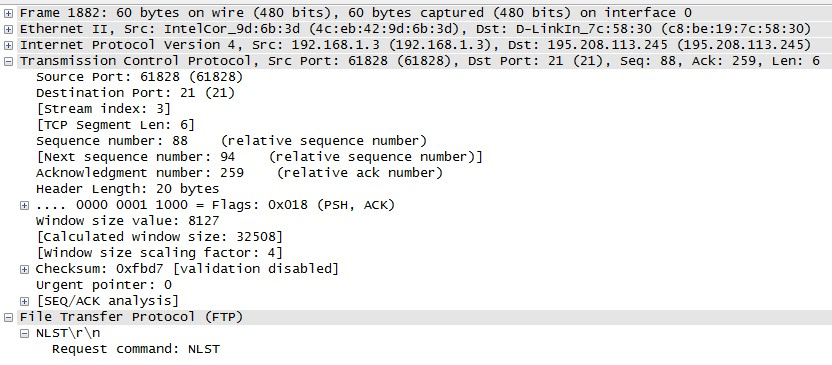
\includegraphics[scale=0.8]{files_req}}
	\caption{Запрос списка файлов}
	\label{img:ftp_act1}
	\end{figure}
	
	
	Далее осуществляется соединение по заданным IP и номеру порта. Запрос на соединения отправляет сервер.
	\begin{figure}[h!]
		\center{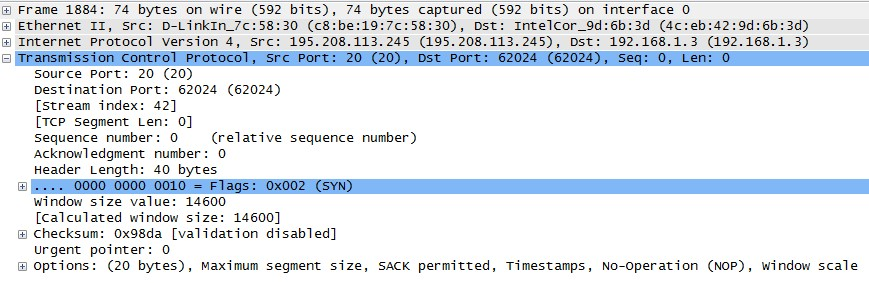
\includegraphics[scale=0.8]{req}}
		\caption{Запрос на соединение от сервера}
		\label{img:ftp_act1}
	\end{figure}
	
	\begin{figure}[h!]
		\center{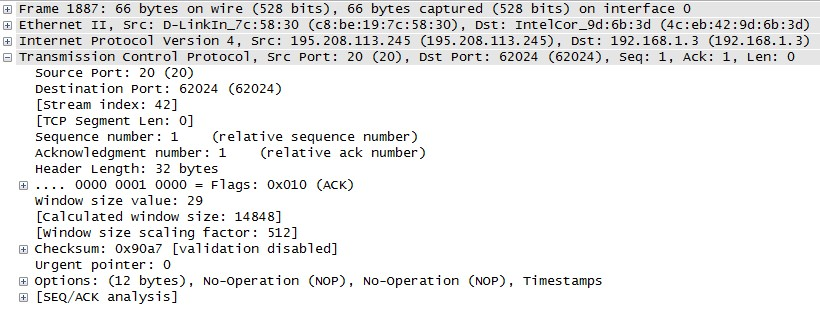
\includegraphics[scale=0.8]{ackn}}
		\caption{Подтверждение установки соединения}
		\label{img:ftp_act1}
	\end{figure}
	
	\newpage
	

	
\subsection{Безопасность протокола}
	FTP-аутентификация, как правило, применяет обычную схему имя пользователя/пароль для предоставления доступа. Имя пользователя посылается серверу в виде команды USER, а пароль - в виде команды PASS. Если предоставленная клиентом информация принята сервером, то сервер отправит клиенту приглашение и начнется сессия. Также, пользователи могут, если сервер позволяет, войти в систему без предоставления учетных данных, но сервером предоставляется лишь ограниченный доступ для таких сессий.
	
	Но также хост FTP-сервиса может предоставить анонимный доступ к FTP. Пользователи обычно входят в систему анонимно, в качестве имени пользователя используется «anonymous». Как правило, пользователей просят прислать адрес электронной почты вместо пароля, никакой тщательной проверки не производится. Многие FTP-хосты, предоставляющие обновления программного обеспечения, поддерживают анонимный доступ.


	\begin{figure}[h!]
	\center{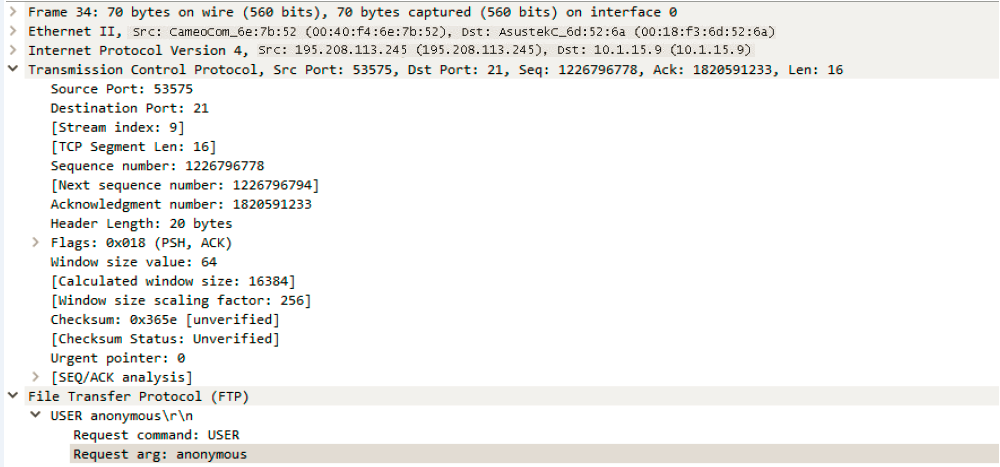
\includegraphics[scale=0.7]{anon}}
	\caption{Пакет с логином для подключения}
	\label{img:ftp_act1}
	\end{figure}
	
	В ответ, сервер прислал пакет с кодом 331.
	\begin{figure}[h!]
	\center{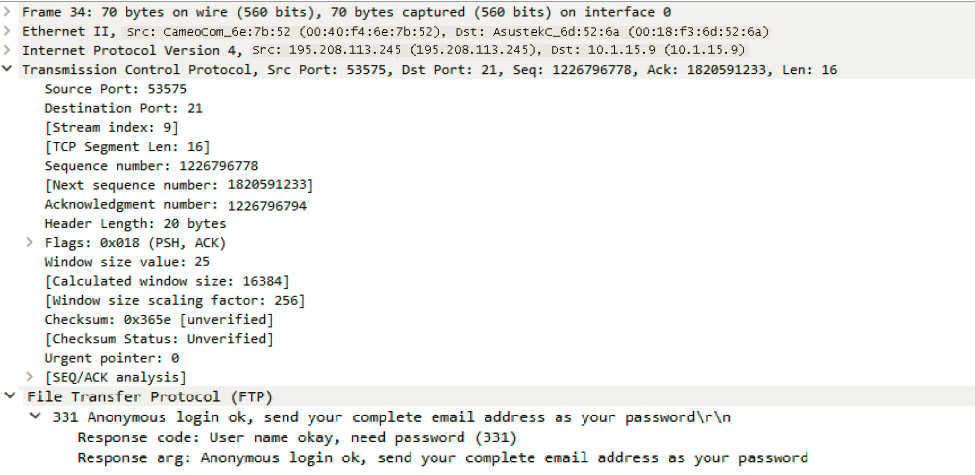
\includegraphics[scale=0.7]{anon2}}
	\caption{Ответ сервера на пакет с логином}
	\label{img:ftp_act1}
	\end{figure}
	
	\newpage
	Вводится пароль и клиент получает пакет с кодом 230, сообщающий об успешной идентификации и воз-
	можности работать дальше.
	
	\begin{figure}[h!]
		\center{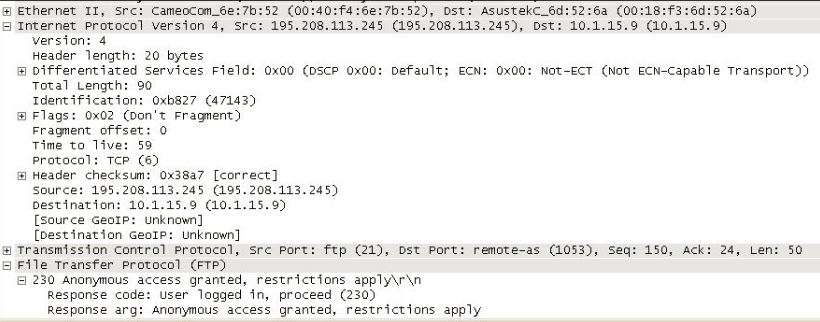
\includegraphics[scale=0.8]{ftp_ack3}}
		\caption{Ответ сервера на пакет с паролем}
		\label{img:ftp_act1}
	\end{figure}
	

\section{Выводы}
В ходе работы были исследованы пакеты протокола FTP. 
FTP отличается от других приложений тем, что он использует два TCP соединения для передачи файла.



\begin{enumerate}
	\item Управляющее соединение устанавливается как обычное соединение клиент-сервер. Сервер осуществляет пассивное открытие на заранее известный порт FTP (21) и ожидает запроса на соединение от клиента. Клиент осуществляет активное открытие на TCP порт 21, чтобы установить управляющее соединение. Управляющее соединение существует все время, пока клиент общается с сервером. Это соединение используется для передачи команд от клиента к серверу и для передачи откликов от сервера. Тип IP сервиса для управляющего соединения устанавливается для получения "минимальной задержки", так как команды обычно вводятся пользователем.
	\item Соединение данных открывается каждый раз, когда осуществляется передача файла между клиентом и сервером. (Оно также открывается и в другие моменты, как мы увидим позже.) Тип сервиса IP для соединения данных должен быть "максимальная пропускная способность", так как это соединение используется для передачи файлов.
\end{enumerate}


FTP не разрабатывался как защищённый (особенно по нынешним меркам) протокол и имеет многочисленные уязвимости в защите. FTP не может зашифровать свой трафик, все передачи — открытый текст, поэтому имена пользователей, пароли, команды и данные могут быть прочитаны кем угодно, способным перехватить пакет по сети.\\
Поэтому часто применяется SFTP — отдельный протокол, основанный на SSH. Его преимуществом является способность использовать защищенное соединение для передачи файлов и навигации по файловой системе на обеих системах — локальной и удаленной.

%\section{Список литературы}
%\begin{itemize}
%	\item Душутина Е.В.  Межпроцессные взаимодействия в операционных системах – СПб, 2014 г, 136 с.
%	\item Душутина Е.В.  Практические вопросы оазработки системных приложений – СПб, 2016 г, 155 с.
%	\item Таненбаум Э., Бос Х. Современные операционные системы. 4-е изд. – СПб.: Питер, 2015 – 1120 с.
%\end{itemize}

\end{document}

